
\section{Galactic Chemical Evolution Models}
\label{outflows:sec:gce}

Our GCE models are adapted from Chapter~\ref{migration}.
These models are deliberately simplified to isolate a comparison between a
model that predicts chemical equilibrium and a model that does not with few
moving parts between them.
We describe the modifications we have made for the sake of this comparison, but
otherwise refer to~\S~\ref{migration:sec:methods} for further information.
Though these are multi-zone models including the effects of stellar migration,
we motivate our parameter selection below using the analytic solutions to
one-zone models from~\citet{Weinberg2017b}.
\par
In Chapter~\ref{migration}, we assigned each stellar population in our model an
``analogue'' from the~\hsim~hydrodynamical simulation~\citep{Christensen2012,
Loebman2012, Loebman2014, Zolotov2012, Brooks2014}, defined to be a randomly
chosen star particle that was born at a similar radius and time.
We simplify this prescription here, instead perturbing stellar populations from
their birth radius by a displacement randomly sampled from a normal
distribution based on arguments in, e.g.,~\citet{Frankel2018}.
The width of this normal distribution increases with age as in, e.g.,
Fig.~\ref{outflows:fig:h277_decomposition} in Chapter~\ref{migration}.
We randomly sample the midplane distances~$\left|z\right|$ according to a
$\text{sech}^2(z / 2h_z)$ distribution~\citep{Binney1987}.
We describe these modifications in greater detail in Dubay et al. (2023, in
prep.).
\par
We retain the nucleosynthesis prescription of Chapter~\ref{migration}, which
focused on O and Fe, though we adopt different values for the parameters
themselves.
These yields are defined as the net mass of some element~$x$ produced over all
events in the units of the progenitor population's mass.
For example, a~$1000$~\msun~cluster will produce exactly 1~\msun~of~$x$ if
the yield is~$y_x = 0.001$.
We adopt the following values:
\begin{itemize}

	\item \ycc{O} = 0.01

	\item \yia{O} = 0

	\item \ycc{Fe} = 0.0008

	\item \yia{Fe} = 0.0014,

\end{itemize}
which are a factor of~$\sim$$2 / 3$ lower than in Chapter~\ref{migration}.
The original yields are appropriate for models in which most massive stars
explode, whereas these modification allow for a portion of massive stars to
collapse directly to black holes~\citep{OConnor2011, Pejcha2015, Gerke2015,
Ertl2016, Sukhbold2016, Adams2017, Basinger2021, Griffith2021b}.
The only remaining differences between these simplified models and those of
Chapter~\ref{migration} are the forms of the SFH (see discussion
in~\S~\ref{outflows:sec:gce:calibration} below).

\subsection{Model Calibration}
\label{outflows:sec:gce:calibration}

We invoke different parameterizations of the mass loading factor
$\eta \equiv \dot{M}_\text{out} / \dot{M}_\star$ as the origin of chemical
equilibrium or lack thereof within the disk lifetime.
This parameter describes how much ISM gas is swept up and ejected in an outflow
due to feedback.
With~$\eta > 0$,~\citet{Weinberg2017b} demonstrate that outflows are a strong
sink term, and as a result it can be adjusted to set the equilibrium abundance.
In Chapter~\ref{migration}, we chose an exponential scaling with radius, namely
\begin{equation}
\eta = \frac{\ycc{O}}{Z_{\text{O},\odot}}
e^{-\grad{O} (\ln 10) (R - R_\odot)} + r - 1,
\end{equation}
such that variations in the equilibrium value corresponded to the observed
metallicity gradient~\grad{O}.
In this scenario, the gradient is much less a prediction of the model than
input, though in detail it can be impacted by processes like stellar migration
and radial gas flows.
To emphasize this feature of this model, we take a constant SFH as opposed to
the fiducial ``inside-out'' SFH from Chapter~\ref{migration}.
\par
The non-equilibrium comparison case is a model in which~$\eta = 0$, which is a
popular choice in GCE models of the MW~\citep[e.g.,][]{Minchev2013,
Minchev2014, Spitoni2019, Spitoni2021}.
Abundances do not reach an equilibrium in these models, instead increasing
until the present day (see, e.g., Fig. 2 of~\citealt{Minchev2013} and Fig. 3
of~\citealt{Spitoni2021}).
In this case, the metallicity gradient arises out of inside-out Galaxy growth
alone.
We clarify that the goal of this comparison is not to empirically distinguish
between~$\eta = 0$ and~$\eta \neq 0$, but rather between models that do and do
not reach an equilibrium abundance within the disk lifetime, which is possible
with either choice of~$\eta$ in principle.
\par
We calibrate the parameters of our non-equilibrium model such that the mode of
the MDF predicted from a one-zone model lines up with the gradient measured
in~\S~\ref{outflows:sec:empirical:gradients}.
The distribution in~$Z$ for some element can be expressed as
\begin{equation}
\frac{dN}{d \ln Z} = Z \frac{dN / dt}{dZ / dt}
\propto \frac{\dot{M}_\star}{(\dot{Z} / Z)},
\end{equation}
after which it follows from differentation and a handful of additional chain
rule substitutions that
\begin{equation}
\frac{d^2N}{d \ln Z^2} \propto \dot{M}_\star
\left(\frac{Z}{\dot{Z}}\right)^2
\left[
\frac{\ddot{M}_\star}{\dot{M}_\star} + \frac{\dot{Z}}{Z} -
\frac{\ddot{Z}}{\dot{Z}}
\right].
\label{outflows:eq:mdf-derivative}
\end{equation}
Herein lies a portion of our motivation for choosing the mode as our summary
statistic in quantifying abundance gradients.
If the form of~$Z(t)$ in a one-zone model is known, either analytically or
numerically, then one can solve for the time at which the peak in the MDF is
produced by setting the quantity in square brackets equal to zero.
\par
In the interest of a simple comparison, we take a single exponential SFH
$\dot{M}_\star \propto e^{-t / \timescale{sfh}}$.
For this choice of SFH, the O abundance in a one-zone model follows from
\citet{Weinberg2017b} as 
\begin{equation}
Z_\text{O}(t) = \frac{\ycc{O}}{1 - r - \tau_\star / \timescale{sfh}}
\left(1 - e^{-t / \bar{\tau}}\right),
\label{outflows:eq:zo-waf17}
\end{equation}
where~$\tau_\star \equiv \Sigma_g / \dot{\Sigma}_\star$ is the star formation
efficiency (SFE) timescale describing the SFR per unit ISM mass,~$r \approx 0.4$
is a correction parameter accounting for the return of stellar envelopes back
to the ISM, and
\begin{equation}
\bar{\tau} \equiv \left(
\frac{1 - r}{\tau_\star} - \frac{1}{\tau_\text{sfh}}
\right)^{-1}.
\label{outflows:eq:taubar-def}
\end{equation}
Computing the necessary time derivatives, combining terms in equation
\refp{outflows:eq:mdf-derivative}, and mapping the time the peak of the MDF is
produced back to the O abundance via equation~\refp{outflows:eq:zo-waf17}
yields the following expression for the position of the mode
\begin{equation}
\text{mode([O/H])} = \log_{10} \left(
\frac{\ycc{O} \timescale{sfh}}{Z_{\text{O},\odot} \tau_\star}
\right).
\end{equation}
\par
In principle, the mode will shift with radius due to changes in
both~$\tau_\star$ and~\timescale{sfh}.
We use a classic single power-law relating the surface densities of gas and
star formation~$\dot{\Sigma}_\star \propto \Sigma_g^N$
\citep[e.g.,][]{Kennicutt1998}.
This approximation allows the SFE timescale to be expressed in terms of radiu
as~$\tau_\star \propto e^{(N - 1) R / R_g}$, where~$R_g$ is the scale radius of
the gas disk.
We now arrive at a relationship between~\timescale{sfh} and radius, calibrated
for this non-equilibrium model:
\begin{equation}
\timescale{sfh} = \tau_{\star,0} \frac{Z_{\text{O},\odot}}{\ycc{O}}
\exp\left[(N - 1)\frac{R}{R_g} + \grad{O} (\ln 10)(R - R_\odot)\right],
\label{outflows:eq:tausfh-radius}
\end{equation}
where~$\tau_{\star,0}$ simply sets the value of~$\tau_\star$ at~$R = 0$,
$Z_{\text{O},\odot}$ is the O abundance in the Sun, and~$R_\odot = 8$ kpc is
the assumed Galactocentric radius of the Sun.
Based on the presence of the central molecular zone in the inner few hundred pc
of the Galaxy~\citep[e.g.,][]{Morris1996, Dahmen1998, PiercePrice2000,
Hatchfield2020} and~\citeauthor{Leroy2008}'s~\citeyearpar{Leroy2008}
measurement of~$\tau_\star \approx 2$ Gyr for purely molecular gas, we
attribute this value to~$\tau_{\star,0}$.
We adopt the commonly used value of~$N = 1.5$ from~\citet{Kennicutt1998}
and~$\grad{O} = -0.06$ kpc$^{-1}$ from our measurements
in~\S~\ref{outflows:sec:empirical:gradients}.
Given these choices, we take~$R_g = 3$ kpc so that~\timescale{sfh} increases
with radius, as expected from inside-out Galaxy formation (for large values
of~$R_g$,~\timescale{sfh} decreases with radius).

\subsection{Model Predictions}
\label{outflows:sec:gce:predictions}

\begin{figure*}
\centering
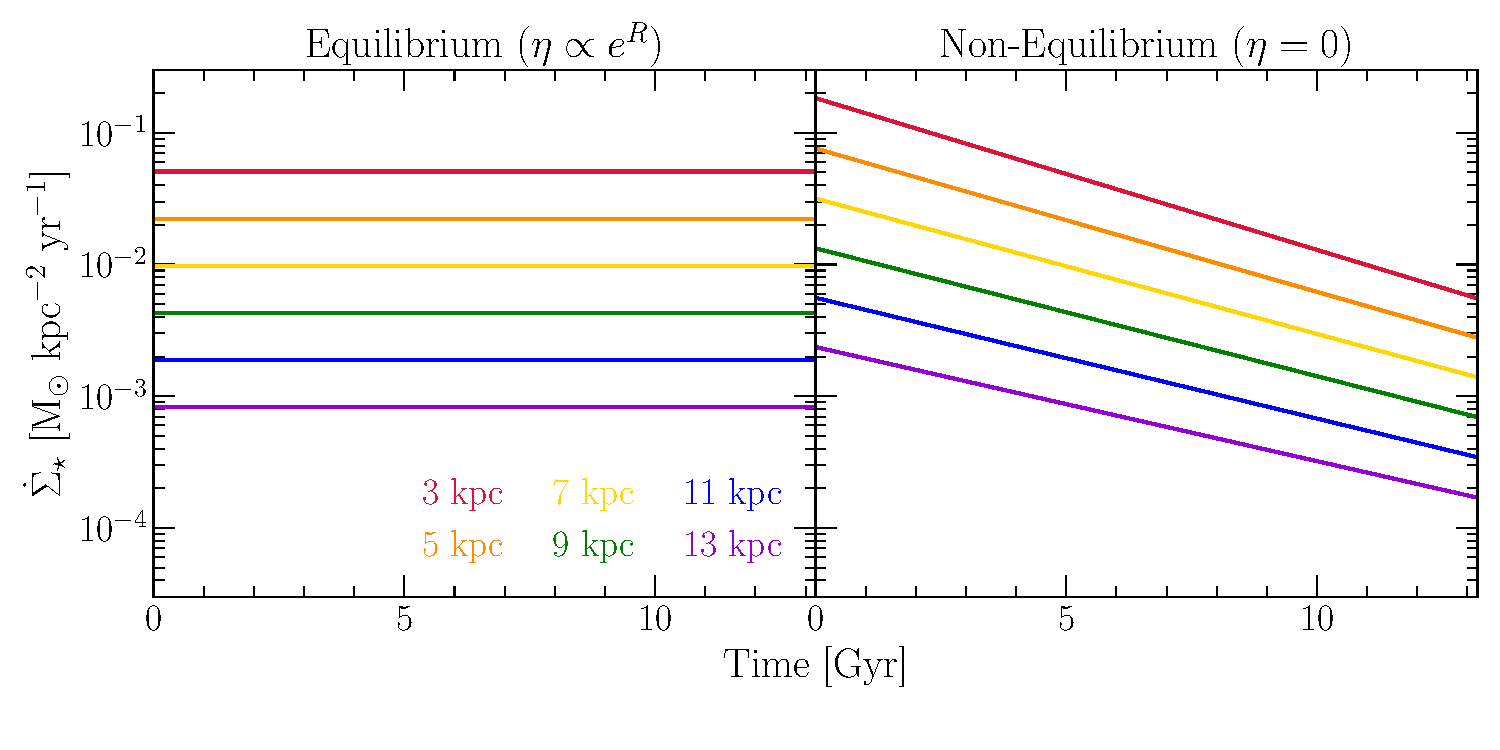
\includegraphics[scale = 0.5]{simplified-examples-sfhs.pdf}
\caption{
SFHs of the~$\eta \propto e^R$ (left) and the~$\eta = 0$ (right) simplified
examples.
Each curve shows the time dependence at a specific radius, color coded
according to the legend.
}
\label{outflows:fig:simplified-examples-sfhs}
\end{figure*}

Fig.~\ref{outflows:fig:simplified-examples-sfhs} shows the SFHs of these
example models.
The e-folding timescale~\timescale{sfh} varies only marginally with radius
($3 - 5$ Gyr across most radii) given our parameter choices (see discussion
at the end of~\S~\ref{outflows:sec:gce:calibration} above).
Fig.~\ref{outflows:fig:simplified-examples} shows the predicted enrichment
histories.
The build up of metals in the ISM is fundamentally different between these two
models.
By intention, the equilibrium model predicts abundances that reach a steady
state at all radii early in the lifetime of the Galactic disk.
In the non-equilibrium model, the metallicity increases monotonically up to the
present day.
There is indeed an equilibrium abundance in the non-equilibrium model, but it
is significantly super-solar and it simply takes much longer than the disk
lifetime to reach it.

\begin{figure*}
\centering
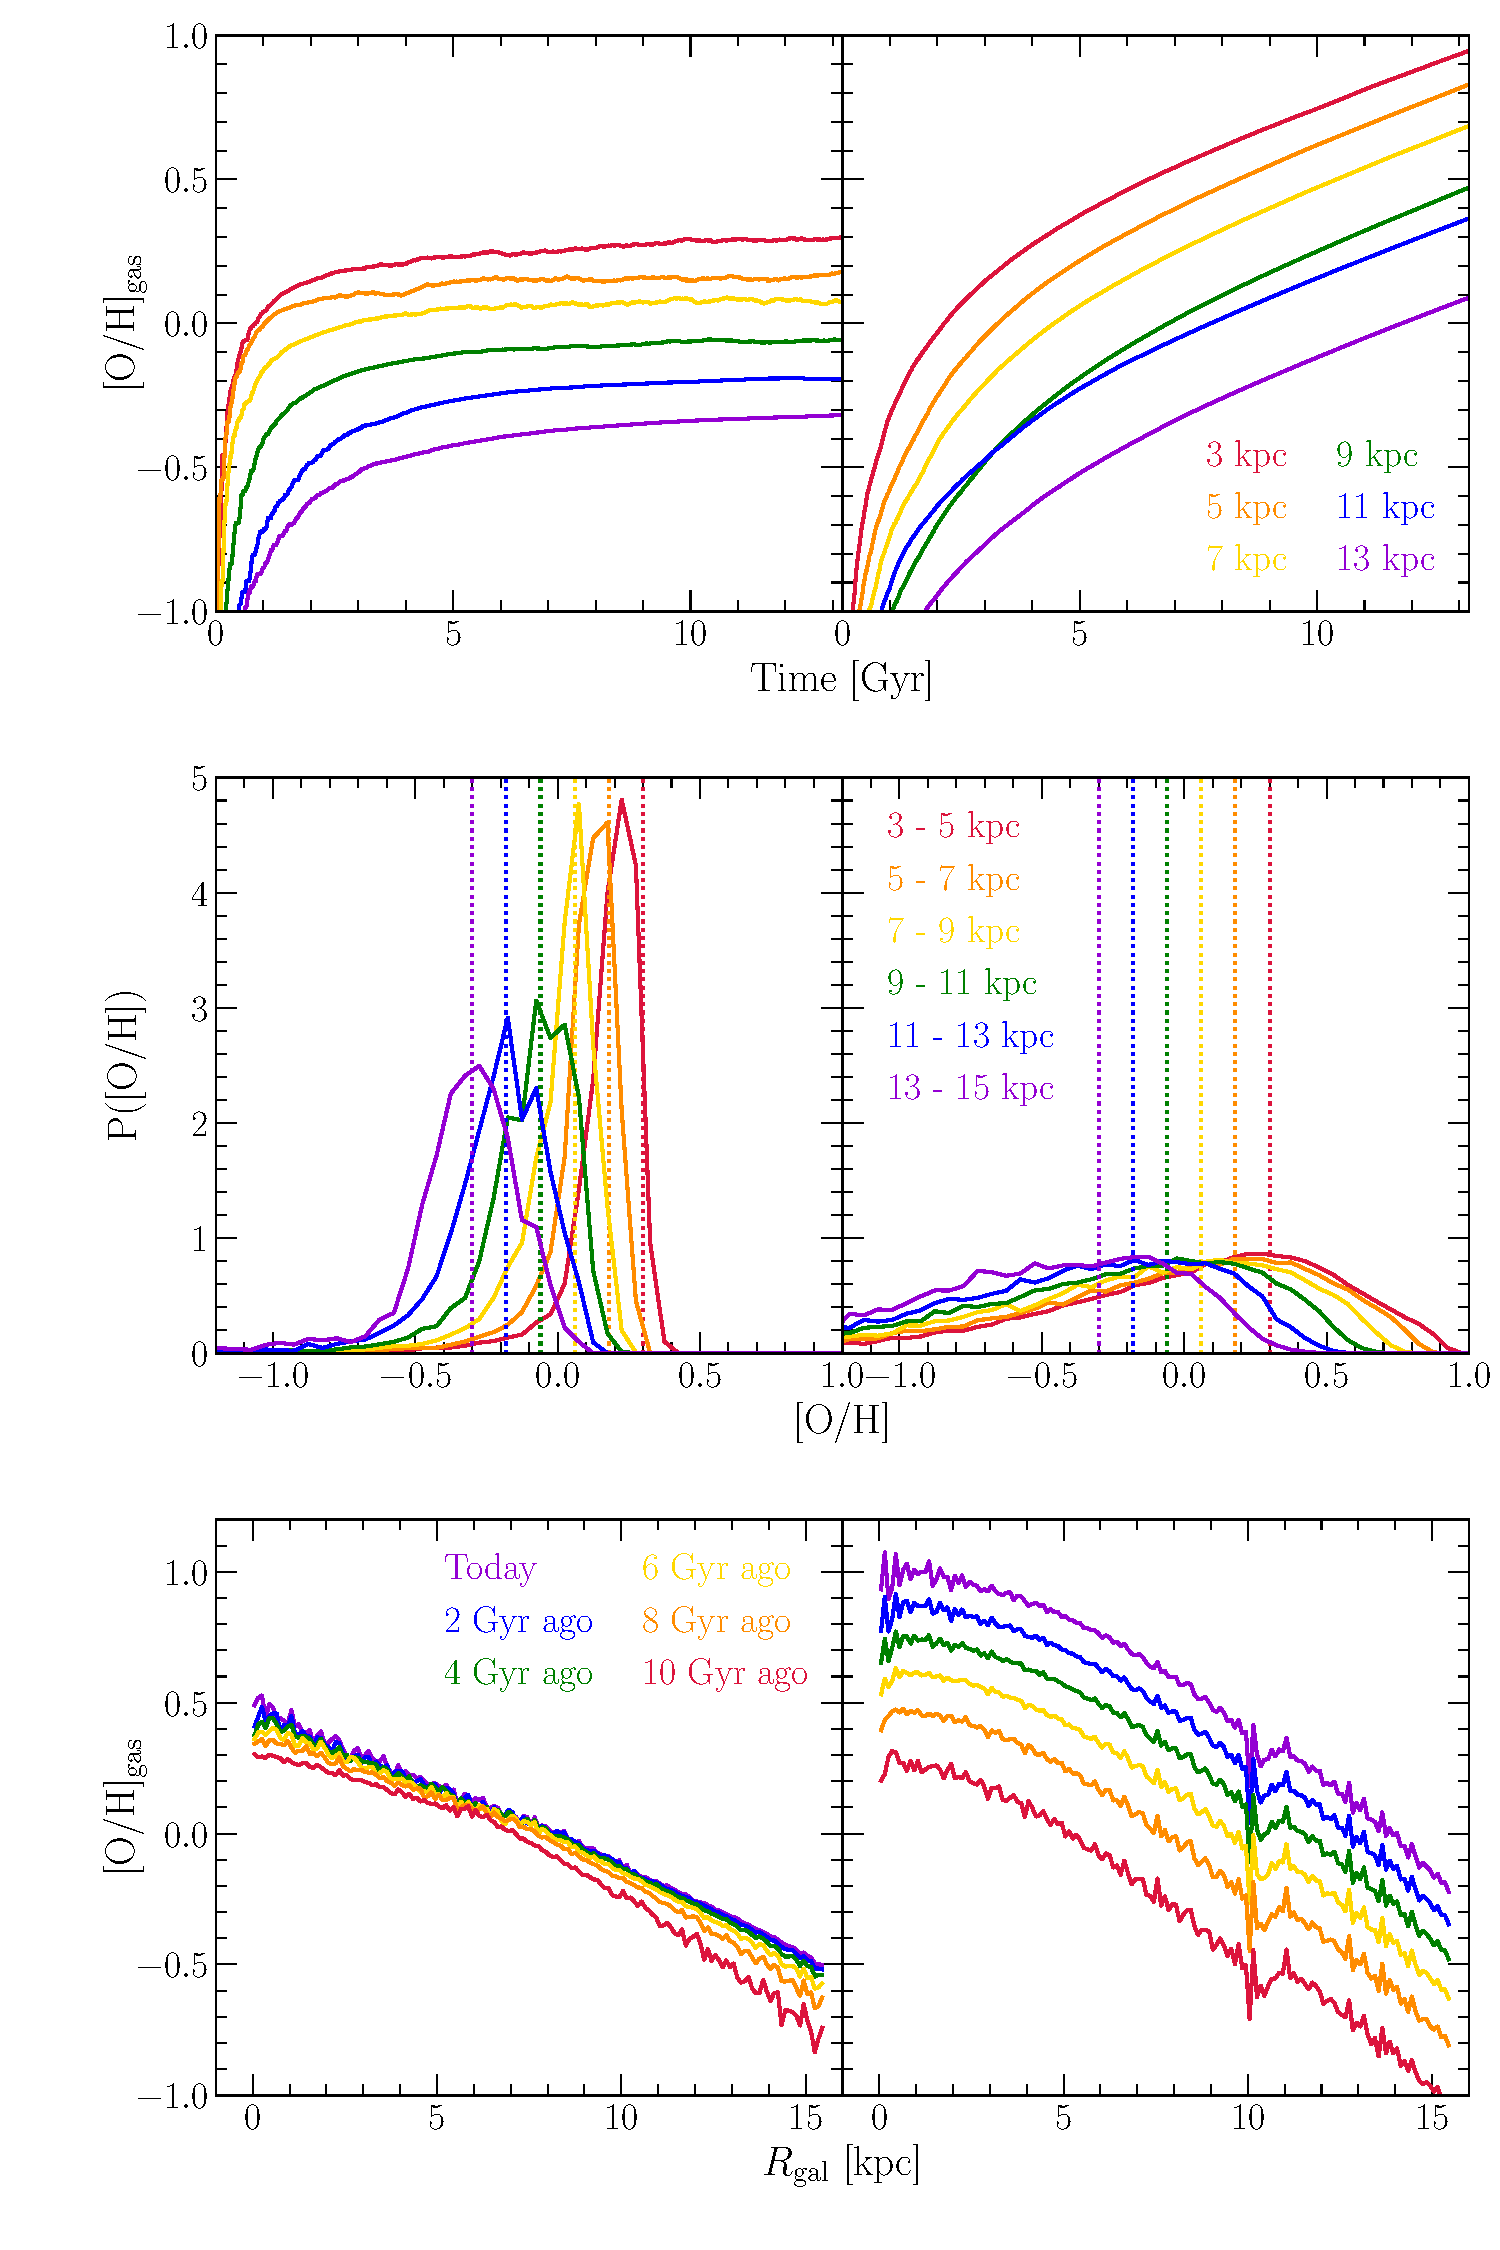
\includegraphics[scale = 0.5]{simplified-examples.pdf}
\caption{
Predicted evolutionary histories of the~$\eta \propto e^R$ (left) and
$\eta = 0$ (right) simplified examples:~\oh~in the ISM at a selection of radii
(top), the distributions in [O/H] in radial bins (middle), and radial
gradients in the gas-phase at snapshots between 2-Gyr intervals (bottom).
Each pair of panels has its own legend identifying the individual curves.
Vertical dotted lines mark the position of the ``target'' gradient with a
slope of~$\grad{O} = -0.06$ kpc$^{-1}$ as measured from our APOGEE sample
in~\S~\ref{outflows:sec:empirical:gradients}.
}
\label{outflows:fig:simplified-examples}
\end{figure*}

These differences in metal build up leave a distinct imprint on the observed
abundance distributions.
The MDFs at all radii are much narrower in the equilibrium model.
This prediction arises because the ISM forms stars at a similar abundance for
most of the disk lifetime, the defining feature of chemical equilibrium.
Otherwise, the ISM simply spends much less time forming stars at one
distinct abundance, resulting in the much broader MDFs seen in the
non-equilibrium model.
The continual build up of metals over time also leads to an increasing
normalization of the abundance gradient, while the chemical equilibrium
scenario predicts a gradient that is largely unchanging.
Both the narrow widths of the MDFs in our APOGEE sample (see
Fig.~\ref{outflows:fig:age-xh-dists}) and the age-independent nature of the
stellar abundance gradient (see Fig.~\ref{outflows:fig:gradxh-fixed-age})
favor the equilibrium model over the non-equilibrium model.
\par
Lastly, we note our final for choosing the mode as our summary statistic in
measuring the abundance gradient.
Vertical dotted lines in the middle panel of
Fig.~\ref{outflows:fig:simplified-examples} note the position of the expected
value of~\oh~from our linear fit to the gradient
in~\S~\ref{outflows:sec:empirical:gradients}.
In both the equilibrium and non-equilibrium models, the MDF peaks close to its
intended position based on our parameter calibration
in~\S~\ref{outflows:sec:gce:calibration} (though it is less obvious in the
non-equilibrium scenario due to the broad nature of the distributions).
Stellar migration enhances the tails of the MDFs in these models, but is not
a strong enough effect to shift the position of the peak.
Since the mean and median are sensitive to the tails of any distribution, they
are therefore impacted by stellar migration while the mode should be largely
uncontaminated.


% Fig.~\ref{outflows:fig:simplified-examples-sfhs} shows the SFHs of these
% example models.
% The e-folding timescale~\timescale{sfh} varies only marginally with radius
% ($3 - 5$ Gyr across most radii), indicating that it is mostly the increase
% in~$\tau_\star$ driving the abundance gradient.
% Fig.~\ref{outflows:fig:simplified-examples} shows the predicted enrichment
% histories.
% The build up of metals in the ISM is fundamentally different between these two
% models.
% In the case of~$\eta \propto e^R$,~\oh~increases quickly at early times at all
% radii, but reaches the equilibrium abundance after~$\sim$$2 - 3$ Gyr in the
% inner disk and~$\sim$$4 - 5$ Gyr in the outer disk.
% With~$\eta = 0$, abundances increase up to the present day.
% There is an equilibrium abundance in this model, but it is significantly
% super-solar, and it simply takes much longer than a Hubble time to reach it.
% \par
% The differences in metal build up leave a distinct imprint on the stellar
% abundance distributions.
% In the equilibrium scenario, the distributions are strongly peaked, whereas
% they are much broader without mass loading.
% In the former, this prediction arises because the ISM forms stars at a similar
% abundance for most of the disk lifetime.
% In the latter, the peak of the MDF occurs at the ``sweet spot'' calibrated
% above, when the rate of star formation becomes too low to populate the upper
% end of the MDF.
% Due to the ongoing build up of metals without mass loading, the MDF is much
% broader.
% The ISM simply spends much less time forming stars at one distinct abundance.
% \par
% The continual build up of metals also leaves distinct features in the gas-phase
% gradient at different snapshots in time.
% The signature left behind on the radial gradient is an increase in the overall
% normalization over time, while the shape remains largely constant.
% The equilibrium scenario, by its very nature, instead produces a gradient that
% evolves very little between redshift~$z \approx 2$ and the present day.
% \par
% Lastly, we note an additional reason for choosing the mode as our summary
% statistic in quantifying stellar abundance gradients.
% The middle row of Fig.~\ref{outflows:fig:simplified-examples} marks the
% expected value of~\oh~from our linear fit to the gradient
% in~\S~\ref{outflows:sec:empirical:gradients}.
% In both models, the MDF peaks extremely close to its intended position.
% The only noticeable exception is the~$R = 3 - 5$ kpc bin in the
% $\eta \propto e^R$ model, though the difference is~$< 0.1$ dex anyway.
% The match between the intended and actual position of the mode is less
% obvious in the~$\eta = 0$ model due to the broad nature of the MDFs, so we have
% zoomed in on these distributions to verify that they do indeed match well.
% At any given radius, stellar migration enhances the metal-rich and metal-poor
% tails of the MDF with stars from small~$R$ and large~$R$, respectively.
% However, the mode is largely unaffected, indicating that its information
% content on the enrichment history in a given Galactic region is relatively
% uncontaminated by migration.
% The median and especially the mean, on the other hand, are sensitive to the
% tails of the MDF.

% \subsection{Calibrating to the Gas-Phase Gradient}
% \label{outflows:sec:calibrated-model}

% We now calibrate a model with~$\eta = 0$ to reproduce the gas-phase gradient at
% the present day.
% While this observable arises as a consequence of the~$\eta \propto e^R$
% specification in Chapter~\ref{migration}, it depends much more strongly on the
% detailed SFH without mass loading.
% To this end, we take the inside-out SFH (see
% equation~\ref{outflows:eq:inside-out-sfh}) and tune~\timescale{rise}
% and~\timescale{sfh} such that the present-day ISM abundances line up with
% \citeauthor{MendezDelgado2022}'s~\citeyearpar{MendezDelgado2022} measurements
% (see Fig.~\ref{outflows:fig:gradxh-gradage} and discussion
% in~\S~\ref{outflows:sec:empirical:gradients}).
% \par
% Drawing on the results of~\S~\ref{outflows:sec:gce:onezone:simple-cases}, the
% build up of O in the ISM will proceed according to the appropriate form
% of~$f_\text{sfh}$ from Table~\ref{outflows:fig:f-sfh-forms}, modulo the impact
% of stellar migration and radial flows.
% As a fiducial choice of parameters, we retain~$R_g = 3$ kpc,
% $\tau_{\star,0} = 2$ Gyr,~$\eta = 0$,~$\grad{O} = -0.06$ kpc$^{-1}$,~$N = 1.5$,
% and~$v_g = 0$ from~\S~\ref{outflows:sec:simplified-example} above.
% Given these choices, the only remaining unknowns before the full time evolution
% of~$Z_\text{O}(t)$ is known are~\timescale{rise} and~\timescale{sfh}.

% \begin{landscape}
% \begin{figure*}
% \centering
% 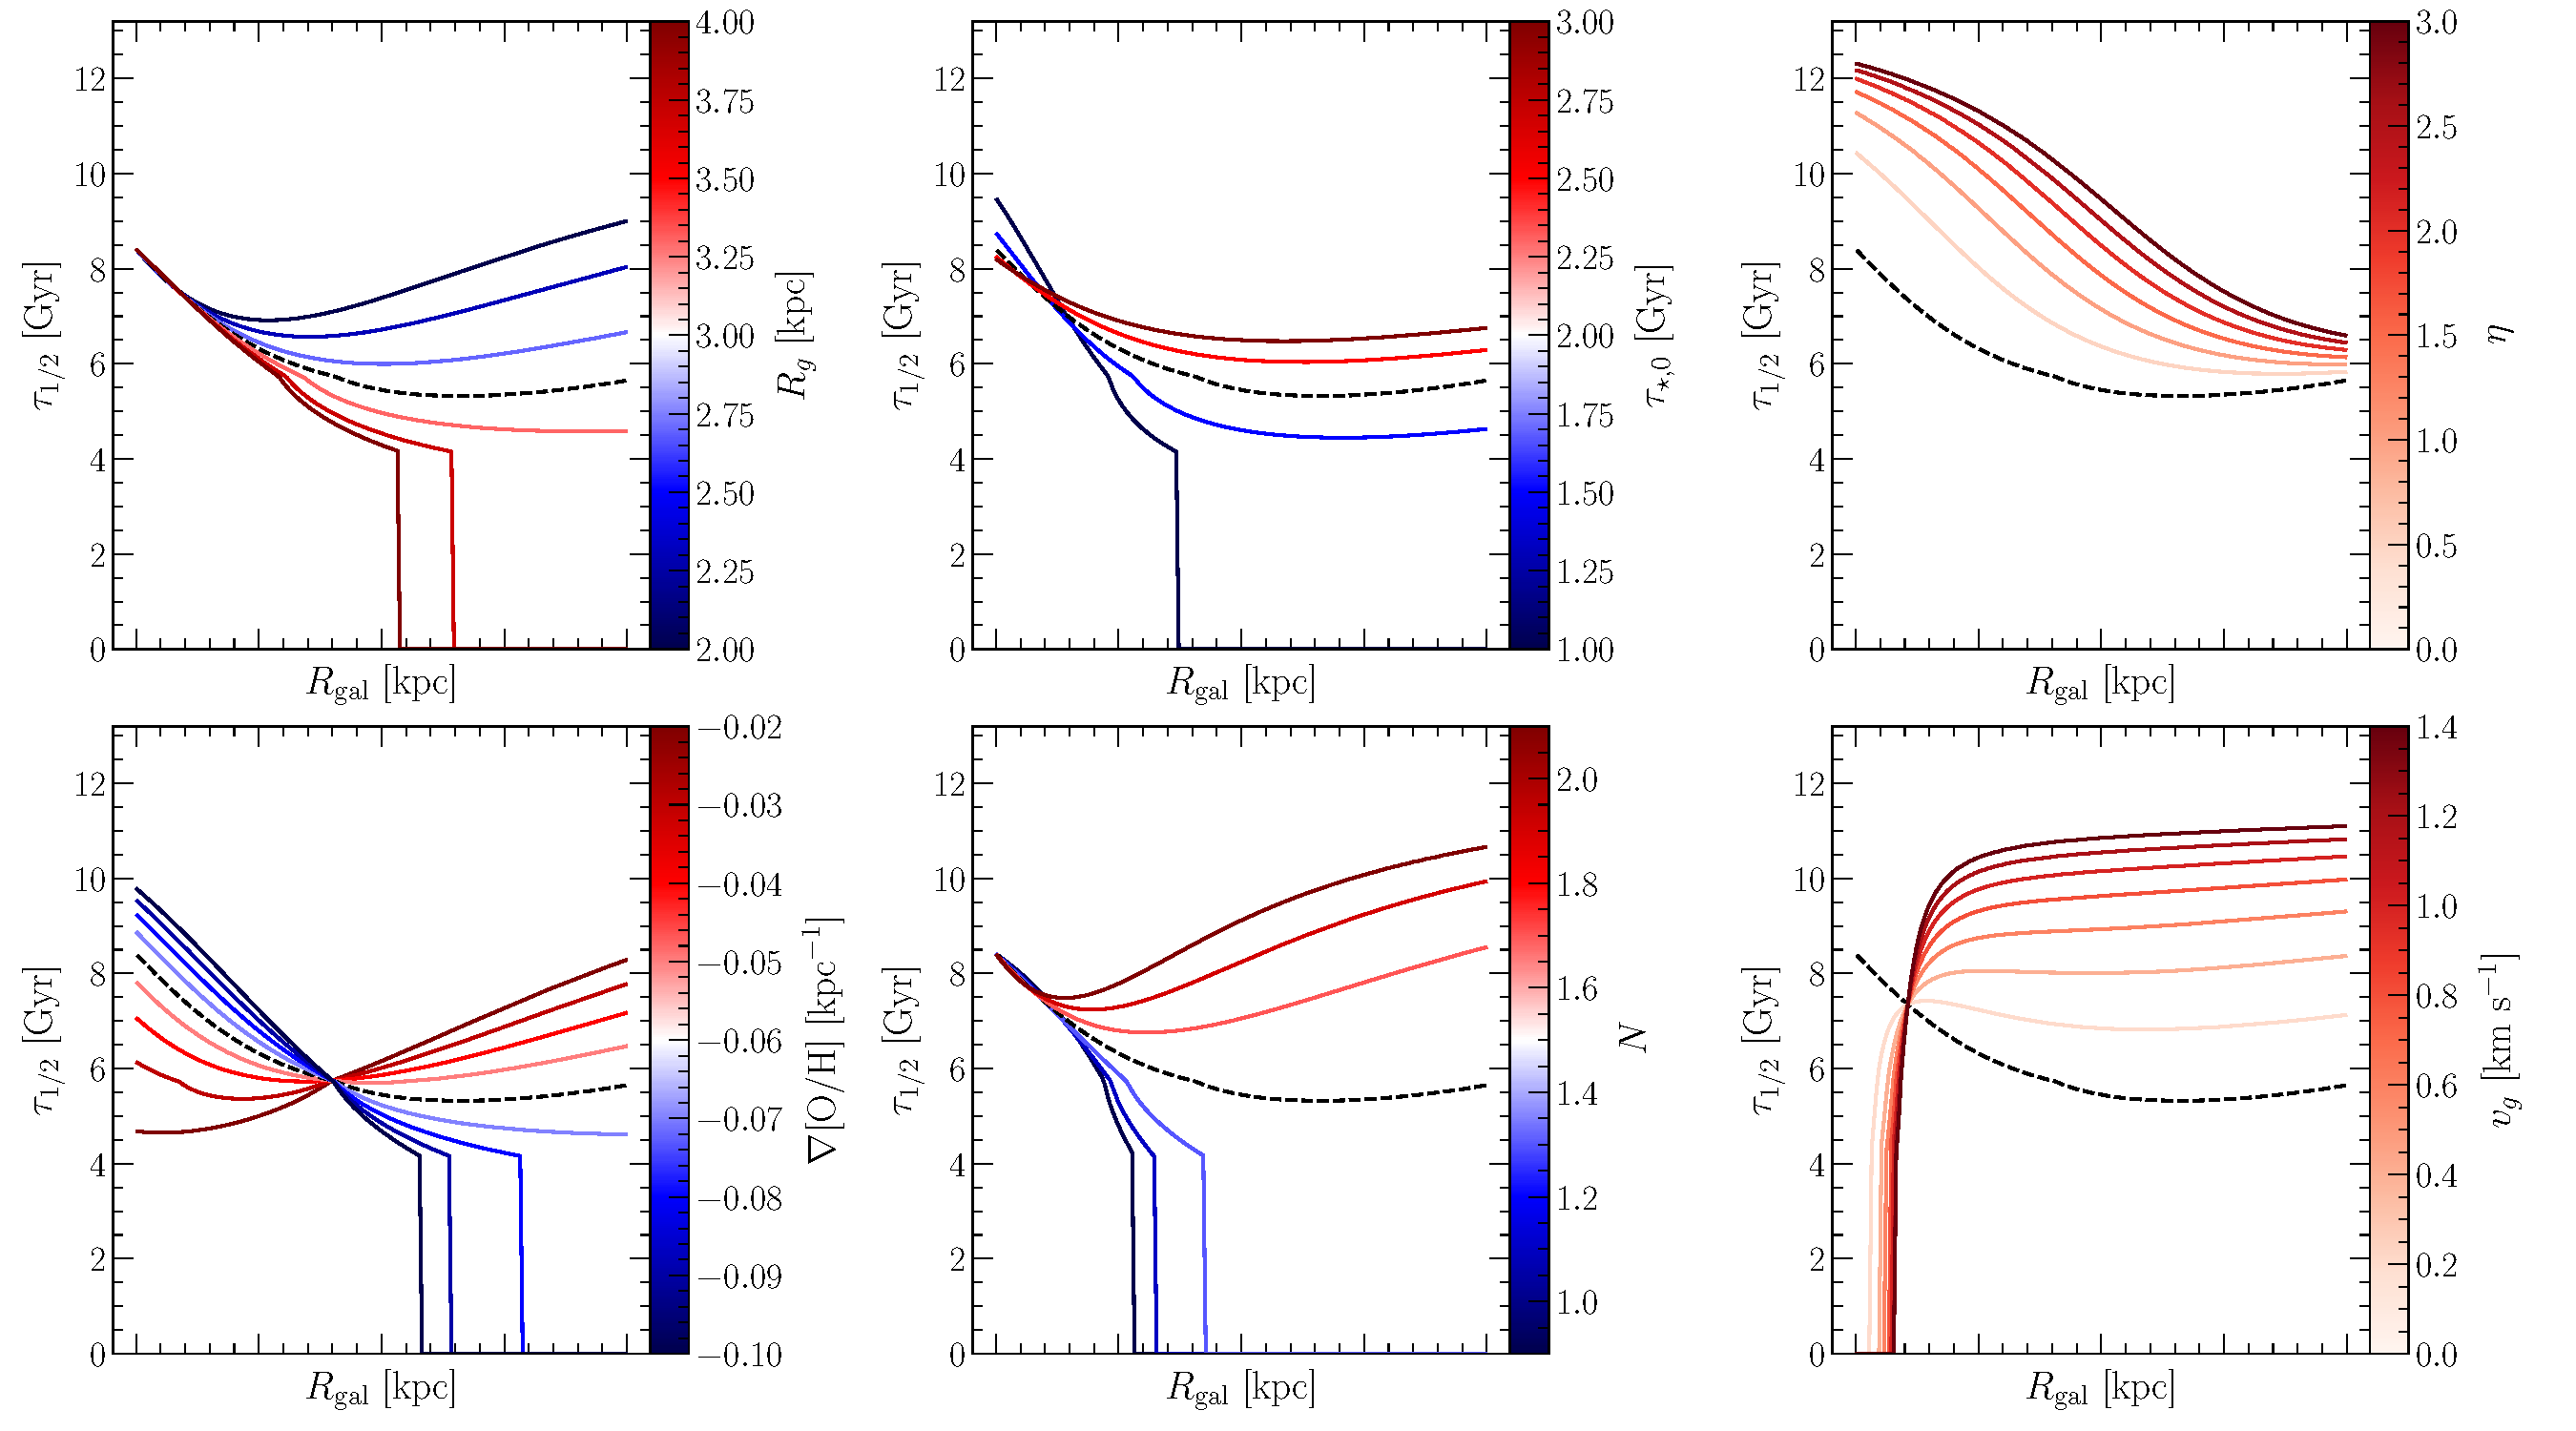
\includegraphics[scale = 0.4]{medage_inputparams.pdf}
% \caption{
% Median age as a function of radius.
% }
% \label{outflows:fig:medage-inputparams}
% \end{figure*}
% \end{landscape}

% Following Chapter~\ref{migration}, we initially set the rise timescale
% to~$\timescale{rise} = 2$ Gyr.
% We then attempt to solve for~\timescale{sfh} via bisection.
% If the value exceeds~$\timescale{sfh} = 200$ Gyr (essentially flat
% at~$t >> \timescale{rise}$), we then hold it fixed there and solve for the
% value of~\timescale{rise}.
% If this value also exceeds~$200$ Gyr, then we conclude that there is no
% physical solution under the given parameter choice.
% We then map~\timescale{rise} and~\timescale{sfh} to the median age of stellar
% populations~$\tau_{1/2}$ by integrating over the implied SFH with an assumed
% disk lifetime of~$\timescale{disk} = 13.2$ Gyr.
% \par
% {\color{red} Potentially move this to a discussion section.}
% Fig.~\ref{outflows:fig:medage-inputparams} shows the results of applying this
% procedure as a function of radius and exploring variations in the individual
% parameters.
% The sensitivity of the predicted age gradient to the input parameters
% underscores a key difference between the~$\eta = 0$ and~$\eta \propto e^R$
% scenarios.
% Without mass loading and variations thereof with radius, the shape of the SFH
% is all there is to vary between Galactic regions.
% If the shape of the SFH (i.e., inside-out galaxy growth) is the primary
% mechanism behind the radial abundance gradient, then it is directly connected
% to the age gradient.
% \par

































% In the case of a single exponential SFH, differentiating
% $\dot{M}_\star \propto e^{-t / \tau_\text{sfh}}$ and
% $f_\text{sfh} = 1 - e^{-t / \taupsi{O}}$ (see
% Table~\ref{outflows:tab:f-sfh-forms}) and solving for the time~$t_\text{max}$
% at which the turnover in the MDF is produced yields
% \begin{equation}
% t_\text{max} = -\taupsi{O} \ln \left(1 - \frac{\timescale{sfh}}{\taupsi{O}}
% \right).
% \end{equation}
% Computing~\oh~based on~$f_\text{sfh}(t_\text{max})$ indicates that the mode
% occurs at
% \begin{equation}
% \text{mode([O/H])} = \log_{10}
% \left(\frac{\ycc{O} \timescale{sfh}}{Z_{\text{O},\odot} \tau_\star}\right).
% \end{equation}
% \par
% In principle, the mode will shift due to changes in both~$\tau_\star$ and
% \timescale{sfh}.
% Since this is a deliberately simplified example, we do not use the three
% component power-law~$\dot{\Sigma}_\star - \Sigma_g$ relationship as in the
% $\eta > 0$ comparison case (see discussion below).
% We instead take a single power-law, enabling a straightforward solution
% for~$\tau_\star$ and therefore~\timescale{sfh} as a function of radius.
% By definition,
% \begin{equation}
% \begin{split}
% \Sigma_g \tau_\star^{-1} &\propto \Sigma_g^N
% \\
% \tau_\star & \propto \Sigma_g^{1 - N}
% \\
% & \propto e^{(N - 1) R / R_g},
% \end{split}
% \end{equation}
% where~$N$ is the power-law index of the~$\dot{\Sigma}_\star - \Sigma_g$
% relation and~$R_g$ is the scale radius of the gas disk.
% Combining terms, solving for~$\timescale{sfh}$, and replacing mode([O/H]) with
% the desired abundance gradient yields the following relationship between
% \timescale{sfh} and~$R$:
% \begin{equation}
% \tau_\text{sfh} = \tau_{\star,0} \frac{Z_{\text{O},\odot}}{\ycc{O}}
% \exp\left[
% (N - 1)\frac{R}{R_g} + \grad{O}(\ln 10)(R - R_\odot)
% \right],
% \label{outflows:eq:tausfh-simplified}
% \end{equation}
% where~$\tau_{\star,0}$ simply sets the value of~$\tau_\star$ at~$R = 0$,
% $Z_{\text{O},\odot}$ is the O abundance in the Sun, and~$R_\odot = 8$ kpc is
% the Galactocentric radius of the Sun.
% We take~$\grad{O} = -0.06$ kpc$^{-1}$ from our measurements
% in~\S~\ref{outflows:sec:empirical:gradients}.
% We adopt~$N = 1.5$ based on the global SFRs and surface densities of
% low-redshift star forming spirals~\citep{Kennicutt1998}.
% Based on the presence of the central molecular zone in the inner few hundred
% pc of the Galaxy~\citep[e.g.,][]{Morris1996, Dahmen1998, PiercePrice2000,
% Hatchfield2020} and~\citeauthor{Leroy2008}'s~\citeyearpar{Leroy2008}
% measurement of~$\tau_\star \approx 2$ Gyr for purely molecular gas, we
% attribute this value to~$\tau_{\star,0}$.
% We take a scale radius of the gas disk~$R_g = 3$ kpc so that~\timescale{sfh}
% increases with radius, as expected from inside-out Galaxy growth
% (equation~\ref{outflows:eq:tausfh-simplified} suggests there is a region of
% parameter space at high~$R_g$ where the timescale decreases with radius).


